
\title{Абстрактная печать по образцу}

\titlerunning{Абстрактная печать по образцу}

\author{Коровянский Алексей Юрьевич}

\authorrunning{A.Ю.Коровянский}

\tocauthor{A.Ю.Коровянский}
\institute{Санкт-Петербургский государственный университет\\
\email{aleksei.korovianskii@student.spbu.ru}}

\maketitle             

\begin{abstract}
test
\end{abstract}

% У введения нет номера главы
\section*{Введение}
Проблема форматирования программного кода актуальна практически в любом проекте по разработке программного обеспечения. К примеру, на этапе сопровождения продукта ``корректное'' форматирование упрощает анализ и рефакторинг кода. Это также актуально при корпоративной разработке, когда возникает необходимость редактирования стороннего кода. Рассмотрим примеры описания одного и того же класса на языке Java (рис.~\ref{uglyCode}, рис.~\ref{formattedCode}).

\setlength{\belowcaptionskip}{-10pt}

%\fvset{frame=lines,framesep=5pt}
\begin{figure}[ht]
%    \begin{pyglist}[language=java,numbers=left,numbersep=5pt]
  \begin{lstlisting}[language=Java]
    import java.util.*;
    public class Numbers {public static void
    main(String[] 
    args) {Scanner numbers = new Scanner(System.in);System.out
    .print("Give me more numbers!");String number = numbers
    .nextInt(); int i = number;     do {i++;System.out.print(i + " ");} 
    while (i < 5);}}
  \end{lstlisting}
%    \end{pyglist}
\caption{Неформатированный код}    
\label{uglyCode}
\end{figure}

%\fvset{frame=lines,framesep=5pt}
\begin{figure}[ht]
%    \begin{pyglist}[language=java,numbers=left,numbersep=5pt]
  \begin{lstlisting}[language=Java]
    import java.util.*;
    public class Numbers {
      public static void main(String[] args) {
        Scanner numbers = new Scanner(System.in);
        System.out.print("Give me more numbers!");
        String number = numbers.nextInt();
        
        int i = number;
        
        do {
            i++;
            System.out.print(i + " ");
        } while (i < 5);
      }
    }
  \end{lstlisting}
%    \end{pyglist}
\caption{Форматированный код}    
\label{formattedCode}
\end{figure}

Представленные фрагменты кода эквиваленты синтаксически и семантически, но с визуальной точки зрения для анализа кода с рис.~\ref{uglyCode} потребуется гораздо больше времени, чем для кода с рис.~\ref{formattedCode}.

Одним из распространенных решений проблемы поддержки принятого стиля форматирования является использование общепроектного стандарта кодирования (СК)~--- набора соглашений, использующихся при написании программного кода~\cite{artOfAgile, indentation}. К сожалению, так как понятие ``корректного'' стиля форматирования субъективно\footnote{У различных компаний отличаются предпочтения форматирования кода на языке Java. Например, существует стиль форматирования, предложенный компанией Oracle (\url{http://www.oracle.com/technetwork/java/index-135089.html}), отличный от стиля форматирования компании Google (\url{https://google-styleguide.googlecode.com/svn/trunk/javaguide.html}).}, поддержка использования стандарта кодирования становится нетривиальной задачей. 

Программные средства, работающие с текстом программ на некотором языке и выполняющие определенные задачи над этими текстами, называются \textit {языковыми процессорами} (ЯП). В частности, задачей ЯП может быть приведение исходного кода к соответствующему стандарту форматирования.

Чаще всего на первом этапе работы ЯП производит синтаксический анализ кода, в результате которого строится древовидное представление программы. В большинстве задач на следующих этапах ЯП работает только с этим представлением. В контексте рассматриваемой проблемы языковой процессор будет проводить обратное преобразование~--- из древовидного представления программы в текстовый. Такое преобразование называется \textit{pretty printing}, а соответствующий инструмент~--- \textit{pretty printer}, далее именуемый принтером. Работа будет вестись с принтерами на основе синтаксических шаблонов и сопоставления с образцом, описанными в~\cite{podkopaev:course, podkopaev:diploma}. В~\cite{podkopaev:diploma} предложена система, которая анализирует образец кода, стиля форматирования которого мы хотим придерживаться, а потом преобразует целевой код в вариант, который соответствует желаемому стандарту кодирования. В контексте упомянутой работы~\cite{podkopaev:diploma} принтеры создаются вручную для каждого конкретного языка. При необходимости поддержки нового языка приходится создавать новый принтер, поскольку исходный использовать невозможно из-за его языкозависимых частей. Однако, некоторые базовые части кода все же можно переиспользовать. Языкозависимыми в предложенных принтерах являются синтаксический анализатор, а также синтаксические шаблоны, неявно содержащие информацию о стиле форматирования конструкций языка. Эти шаблоны создаются после анализа образца кода, стиля которого мы хотим придерживаться. Таким образом, предложенные принтеры решают проблему форматирования кода программ для конкретного языка, но, при необходимости расширения множества поддерживаемых языков, приходится создавать новые принтеры с нуля.

\section{Постановка задачи}

Целью работы является исследование вопроса генерации принтеров, использующих синтаксические шаблоны и сопоставление с образцом~\cite{podkopaev:diploma}. 
Это позволит минимизировать время создания новых принтеров для поддержки новых языков программирования.
Для достижения данной цели были поставлены следующие задачи.
\begin{itemize}
\item Исследовать структуру классов описаний синтаксических шаблонов, для создания системы, позволяющей задать все необходимые параметры для генерации языкозависимой части принтеров.
\item Реализовать генератор принтеров, использующих синтаксические шаблоны и сопоставление с образцом.
\item В рамках апробации метода сгенерировать принтеры для языков Java и Haskell.
\end{itemize}

\section{Обзор существующих решений}
Первое общее решение для описания принтеров было сформулировано Дереком Оппеном~\cite{oppen}. Он описал языконезависимый алгоритм, работающий над последовательностью \textit{блоков} строк. Входной поток разделен специальными объектами (блочные разделители и пробелы). Эти объекты определяют в каком месте может быть осуществлен перенос строки.

Дерек Оппен также ввел понятие \textit{условного форматирования} для поддержки различных вариантов форматирования, когда блок не может поместиться на одну строку. Условное форматирование позволяет, в зависимости от выбранного режима, расставлять переносы тем или иным образом. Блоки определяются для строк любых языков, поэтому основная цель алгоритмов на основе предложенного Оппеном~--- привести исходный текст к блочному виду. Современные принтеры используют также алгоритмы форматирования на основе \textit{box--структур}~--- альтернативе блокам Оппена~\cite{oppenlike:mikelsons, box:knuth}. Существует язык PPML~\cite{oppenlike:morcos}, который определяет синтаксис на основе box--структур для задания форматирования отображаемого текста. Этот язык использует различные варианты box--структур для различных стилей форматирования, например h-box--структуры для горизонтального форматирования и v-box--структуры для вертикального форматирования.

Существует множество алгоритмов, основанных на алгоритме Оппена~\cite{oppenlike:rose, oppenlike:mikelsons, oppenlike:rubin, oppenlike:morcos, oppenlike:brand, oppenfunc:swierstra, oppenfunc:hughes, oppenfunc:wadler}. К сожалению, условное форматирование приводит к экспоненциальному росту количества вариантов форматированных текстов. Традиционные алгоритмы рассматривают лишь некоторое подможество вариантов результирующих текстов, чтобы минимизировать время работы. 

Оппен в работе~\cite{oppen} разделяет принтеры на две части. Первая часть переводит исходный текст к блочному-языконезависимому виду. Эта часть является языкозависимой в принтере. Вторая часть работает с текстом, представленным в блочном виде, и возвращает форматированный результат. Таким образом, языконезависимость принтеров достигается за счет генерации первой части принтера для некоторых языков.

Конкретные предпочтения форматирования описываются в языкозависимой части принтера вручную~\cite{jokinen, oppenlike:morcos}. Также возможна генерация этой части на основе грамматики языка с добавленными правилами форматирования~\cite{boulton, oppenlike:rose, oppenlike:rubin}.

Возможна генерация языкозависимой части только лишь на основе грамматики языка, не указывая правила форматирования. Принтер, работающий на основе этого подхода, описан в~\cite{oppenlike:brand}. В этой работе задается базовый стиль форматирования, а для его изменения нужно редактировать сгенерированный код принтера. Это же является основным недостатком этого подхода, поскольку пользователь обязан разбираться в исходном коде принтера, чтобы задать специфический стиль форматирования.

В основном, алгоритмы~\cite{jonge, jokinen, jackson} базируются на идеях, предложенных Оппеном. Главное отличие таких алгоритмов заключается в способе генерации первой части принтера. Например, в работе Матти Йокинена~\cite{jokinen} в качестве входных данных используются потоки, состоящие из правил форматированния и непосредственно текста программ. Правила форматирования также можно включить в описание грамматики языка. Автор утверждает, что подход обладает низкой выразительностью, поскольку синстаксис правил форматирования сильно ограничен, но при этом позволяет максимально упростить взаимодействие с пользователем. Иной способ представлен в работе Стоуни Джексона~\cite{jackson}. В его работе предлагается создавать метки, определяющие правила форматирования непосредственно при работе с абстрактным синтаксическим деревом программы. Автор реализовал генератор, преобразующий абстрактное синтаксическое дерево в дерево, содержащее пометки о форматировании его узлов.

Существует упрощенный подход к ``генерации'' принтеров. В нем изначально формулируется некоторое множество стилей форматирования. Пользователь же задает параметры для определения нужного стиля из подготовленного множеста, после чего генериуется принтер соответствующий заданным параметрам. К сожалению, у такого подхода очень низкий уровень выразительности. Этот подход лежит в основе работы~\cite{blaschek}.

\section{Описание используемых инструментов}
В качестве основы для генерации было решено использовать принтер, описанный в~\cite{podkopaev:diploma}. Предложенная система работает на основе сравнения с образцом и синтаксических шаблонов. Это значит, что, в отличии от всех перечисленных решений, система автоматически выделяет стиль форматирования из эталонного образца кода. То есть пользователю не нужно самостоятельно задавать правила форматирования, а достаточно указать ``идеальный образец''. 

Под \textit{синтаксическими шаблонами} понимаются данные, сопоставляя которые с переданным на печать синтаксическим деревом, создается текстовое представление этого дерева. Синтаксический шаблон неявно содержит конкретный вариант форматирования некоторой структуры языка. Фактически шаблоны представляют из себя размеченное дерево разбора некоторой синтаксической конструкции, в котором по каждой метке можно понять ограничения на представление соответствующих поддеревьев, а также описание того, как нужная раскладка поддерева должна быть вставлена в шаблон. На рис.~\ref{ifTemplate} можно увидеть текстовое представление синтаксического шаблона. Обозначения ``@NAME'' в ходе работы с синтаксическим шаблоном заменяются на соответствующие текстовые представления поддеревьев конструкции. Расположение всех ключевых слов, скобок, пробелов, переносов строк в шаблоне фиксировано. То есть используя синтаксический шаблон, имеющий текстовое представление с рис.~\ref{ifTemplate}, вне зависимости от текстового представления, например, поддерева ``condition'', закрывающая круглая скобка будет всегда стоять непосредственно после последнего символа этого поддерева.

\fvset{frame=lines,framesep=5pt}
\begin{figure}[ht]
%    \begin{pyglist}[language=java,numbers=left,numbersep=5pt]
\begin{lstlisting}[language=Java]
    if(@COND) {
        @THEN_BRANCH
    }
    else {
        @ELSE_BRANCH
    }
\end{lstlisting}
%    \end{lstlisting}

\caption{Пример текстового представления синтаксического шаблона структуры ``\lstinline{if}''}    
\label{ifTemplate}
\end{figure}

В начале работы указанный принтер анализирует идеальный образец кода и на основе этого образца создает шаблоны структур языка. После создания шаблонов происходит переформатирование стилистически некорректного кода, в процессе которого идет поиск подходящих шаблонов. Если подходящий шаблон был найден, то генерируется целевой программный код, то есть код, который стилистически соответствует идеальному образцу.

В принтере присутствуют \textit{классы описаний шаблонов}, которые определяют для каждой синтаксической конструкции языка какими могут быть ее шаблоны. В них содержатся все возможные метки шаблона, метод для дополнительной проверки применимости шаблона, метод для создания нового экземпляра шаблона, а также методы для работы с поддеревьями конструкции. На этапе анализа идеального образца принтер использует эти классы для создания набора синтаксических шаблонов. Во время работы со стилистически некорректным кодом для каждой распознанной структуры создается набор меток, подобный тому, что определялся для созданных шаблонов. Для генерации этого набора также используются классы описаний шаблонов.

Метки в классах описаний шаблонов однозначно определяют какие варианты соответствующей структуры могут встречаться в языке и чаще всего их столько же, сколько и поддеревьев у заданной структуры. Например, описанию шаблона условной структуры ``\lstinline{if}'' языка Java сопоставляется набор меток: ``\lstinline{condition}``, ``\lstinline{then}``, ``\lstinline{else}''. Причем в описании оговаривается, что для корректности шаблона метки ``\lstinline{condition}'' и ``\lstinline{then}'' являются обязательными, а метки ``\lstinline{else}'' может и не быть. Такое описание порождает два вида шаблонов структуры ``\lstinline{if}''~--- с альтернативной веткой и без нее. Одной и той же структуре может соответствовать несколько шаблонов. Например, образцы кода с рис.~\ref{ifVariants}, порождают два шаблона для структуры ``\lstinline{if}'' без альтернативной ветки и ни одного шаблона для структуры ``\lstinline{if}'' с альтернативной веткой. Это означает, что при получении целевого кода, создастся несколько вариантов и, исходя из критериев оптимальности\footnote{Например, вариант форматирования кода может считаться оптимальным, если, при заданном ограничении ширины вывода, он располагается на минимальном количестве строк.}, выберется наилучший из них. Таким образом, для генерации описаний шаблонов необходимо определить набор меток шаблонов~--- по одной метке на каждое поддерево структуры, а также, например, обязательно ли наличие данной метки для корректности структуры.

\fvset{frame=lines,framesep=5pt}
\begin{figure}[ht]
\noindent\begin{minipage}{.45\textwidth}
    \begin{lstlisting}[language=Java]
    ...
    if(x > 3) {
      return true;
    }
    
    ...
    \end{lstlisting}
\caption*{a)}    
\end{minipage}\hfill
\begin{minipage}{.45\textwidth}
    \begin{lstlisting}[language=Java]
    ...
    if(x > 2) 
    { 
      return false; 
    }
    ...
    \end{lstlisting}
\caption*{b)}    
\end{minipage}
\caption{Различные варианты форматирования структуры ``\lstinline{if}'' языка Java}    
\label{ifVariants}
\end{figure}

На этапе форматирования принтер применяет набор созданных шаблонов к обрабатываемому коду. Под \textit{применением шаблона} понимается замена фрагмента обрабатываемого кода текстовым представлением синтаксического шаблона для этого фрагмента, в котором все параметры ``@NAME'' заменены текстовыми представлениями соответствующих поддеревьев. Для определения соответствия шаблона какой-либо конструкции используется его набор меток, который является подмножеством меток, определенных в классе описания шаблонов. То есть на этапе форматирования принтер для каждой конструкции генерирует некоторый набор меток, который после этого сравнивается с наборами меток каждого синтаксического шаблона. При совпадении меток разрешается применить найденный шаблон к соответствующему фрагменту кода.

В контексте поставленной задачи необходимо выделить языкозависимые части принтера. Языкозависимыми частями в этом принтере являются шаблоны и синтаксический анализатор. Поскольку принтер был разработан как плагин для IntelliJ IDEA, то был использован уже реализованный в этой среде синтаксический анализатор. Далее мы также будем считать, что синтаксический анализатор уже реализован. Таким образом, в первую очередь необходимо исследовать методы генерации описаний шаблонов принтера. 

Для разработки был выбран язык Kotlin. Kotlin\footnote{\url{http://kotlin.jetbrains.org}}~--- это функциональный, объектно-ориентированный, компилируемый в JVM-байткод и JavaScript язык, разрабатываемый компанией JetBrains\footnote{\url{http://jetbrains.org}}. Основной причиной выбора этого языка является совместимость с представленным принтером, который был разработан на этом же языке. Также использование Kotlin позволяет работать с множеством готовых модулей языка Java из-за их совместимости.  

\section{Реализация}
Необходимо определить какими параметрами можно однозначно задавать классы описаний шаблонов. После этого возможно разработать систему описания шаблонов, по которой генерировать языкозависимую часть принтера. Разработанный генератор можно использовать для создания принтеров конкретных языков. В рамках апробации предлагается генерировать принтеры для языков Java и Haskell.

\subsection{Структура для генерации классов описаний шаблонов}

Для однозначного определения соответствия конкретного шаблона к фрагменту исходного кода необходима информация о наборе меток этого фрагмента, а также какой структуре в контексте синтаксического анализа этот фрагмент соответствует\footnote{Например, шаблоны структур ``\lstinline{while}'' и ``\lstinline{do-while}'' могут иметь одинаковый набор меток, поэтому, для определения какой из них необходимо применить к анализируемому фрагменту, нужна также информация о соответствии шаблона, например, структуре ``\lstinline{WHILE}''.}. Синтаксический анализатор предоставляет информацию о некоторой структуре, после этого для данной структуры запрашиваются все шаблоны. Далее среди всех шаблонов для этой структуры выбираются те, набор меток которых совпадает с анализируемым фрагментом. То есть информация о соответствии шаблона конкретной структуре в контексте синтаксического анализатора должна быть указана в классах описания шаблонов и, следовательно, это должно быть одним из параметров системы для генерации этих классов. Иным параметром системы должен быть список меток для описания шаблонов. Этот список можно получить из списка поддеревьев структуры, поэтому в итоговой системе список меток явно не указывается. Также для генерации понадобится информация о методе создания экземпляра класса структуры из ее текстового представления. Этот метод нужен для создания синтаксических шаблонов из идеального образца. Фактически в этих методах используются функции синтаксического анализатора, поэтому чаще всего достаточно указать лишь название необходимой функции анализатора. 

С точки зрения необходимых методов для генерации вариантов текста классы описаний шаблонов можно разделить на содержащие списочные поддеревья и не содержащие. Например, структура ``вызов метода'' имеет поддерево ``список аргументов''. Нельзя применить такой же алгоритм создания шаблонов к такому элементу, как и к элементу без списочных поддеревьев, поскольку необходимо задать весь набор меток шаблона. В этом случае одинаковые структуры с различным количеством элементов в списочных поддеревьях будут иметь различные шаблоны, что противоречит нашей концепции\footnote{Эта ситуация возникнет, если обрабатывать элементы списочных поддеревьев абсолютно также, как и любое другое поддерево. То есть создавать метку на каждый элемент списка.}. Поэтому классы описаний шаблонов для списочных элементов будут иметь отличный набор методов от обычных элементов, и для их генерации необходимо либо иметь встроенное в генератор решение, либо добавлять исходный код методов для обработки таких поддеревьев в качестве входных данных генератору. 

В контесте рассматриваемой проблемы актуален также вопрос о переиспользовании классов описаний шаблонов для различных языков. Если немного модифицированный класс описания шаблонов, например, для конструкции ``\lstinline{if}'' подходит для многих языков, то необходимость в генерации новых классов для этой конструкции исчезает. К сожалению, в силу особенностей синтаксиса языков переиспользовать шаблоны практически невозможно. Особенно это проявляется в языках с двумерным синтаксисом, где применение стиля форматирования, например, языка Java может порождать синтаксически некорректный код. Однако, для более схожих языков, например, Java и C\# переиспользовать некоторые классы возможно.

В качестве входных данных для генератора было решено использовать набор XML-файлов с заданными параметрами для каждой компоненты языка. Эти файлы содержат всю необходимую информацию для генерации классов описаний шаблонов. Основной сложностью является создание достаточно простой системы параметров, чтобы пользователь затрачивал минимальное количество времени на их задание, и при этом достаточно гибкую, для возможности генерации большего множества компонент.

На рис.~\ref{XSD-scheme} показана XSD-схема предложенной системы задания классов описаний шаблонов. В каждом XML-файле описывается объект ``component''. Для каждого объекта ``component'' необходимо указать его имя, соответствующий ему класс в синтаксическом анализаторе, название метода фабрики элементов языка для создания экземпляра конструкции из текста. Необязательными параметрами являются перечисление предков класса, расширяющих его функционал, а также список специфических модулей, необходимых для корректной работы. Указание списка предков класса может быть нужно, если используется некоторое готовое решение для работы с шаблонами. Например, для структуры, отвечающей за арифметические выражения, может быть указан класс предок, содержащий определение приоритета операций. Обычно, при использовании готовых решений, также придется описывать работу с ними непосредственно в XML-файле. Для поддержки такого функционала в генератор была добавлена возможность внедрения готового исходного кода в генерируемый текст. Исходный код может быть включен в атрибуты с именем ``specificCode''. По представленной XSD-схеме можно увидеть, что такой атрибут есть практически у всех элементов объекта ``component''.

В объекте ``component'' перечисляются параметры для методов обработки синтаксических шаблонов, а также список поддеревьев структуры. Каждое поддерево представляется объектом ``subtree''. У этого объекта необходимо указывать имя, название метода синтаксического анализатора для доступа к этому поддереву, является ли это поддерево отдельным функциональным блоком, необходимо ли поддерево для корректности структуры, нужно ли учитывать количество строк в поддереве (``isEverywhereSuit''), состоит ли поддерево из одного элемента или представляет из себя список. Также для каждого метода работы с поддеревом можно указать код для дополнительной обработки, например, если поддерево представляет из себя список, то нужно указать способ соединения его элементов.

\fvset{frame=lines,framesep=5pt}
\begin{figure}[H]
\begin{lstlisting}[language=xml]
<xs:element name="component">
  <xs:complexType>
    <xs:sequence>
      <xs:element name="subtree" maxOccurs="unbounded" 
                  minOccurs="0">
        <xs:complexType mixed="true">
          <xs:sequence>
            <xs:element name="getCode" 
                        maxOccurs="1" 
                        minOccurs="0">
              <xs:attribute type="xs:string" name="foldFunction"/>
              <xs:attribute type="xs:string" name="specificCode"/>
            </xs:element>
            <xs:element name="prepCode" maxOccurs="1" minOccurs="0">
              <xs:attribute type="xs:string" name="specificCode"/>
            </xs:element>
            <xs:element name="addCode" maxOccurs="1" minOccurs="0">
              <xs:attribute type="xs:string" name="specificCode"/>
            </xs:element>
          </xs:sequence>
          <xs:attribute type="xs:string" name="name"/>
          <xs:attribute type="xs:string" name="psiGetMethod"/>
          <xs:attribute type="xs:string" name="isCodeBlock"/>
          <xs:attribute type="xs:string" name="isRequired"/>
          <xs:attribute type="xs:string" name="isEverywhereSuit" 
                        use="opt"/>
          <xs:attribute type="xs:string" name="hasSeveralElements" 
                        use="opt"/>
        </xs:complexType>
      </xs:element>    
      <xs:element name="getNewElement" maxOccurs="1" minOccurs="0">
        <xs:attribute type="xs:string" name="specificCode"/>
      </xs:element>
      <xs:element name="updateSubtrees" maxOccurs="1" minOccurs="0">
        <xs:attribute type="xs:string" name="specificCode"/>
      </xs:element>
    \end{lstlisting}
\end{figure}
\fvset{frame=lines,framesep=5pt}
\begin{figure}[H]
    \begin{lstlisting}[language=xml]
      <xs:element name="specCode" maxOccurs="1" minOccurs="0">
        <xs:attribute type="xs:string" name="specificCode"/>
      </xs:element>
      <xs:element name="isTemplSuit" maxOccurs="1" minOccurs="0">
        <xs:attribute type="xs:string" name="specificCode"/>
      </xs:element>
      <xs:element name="getTemplate" maxOccurs="1" minOccurs="0">
        <xs:attribute type="xs:string" name="specificCode"/>
      </xs:element>
      <xs:element name="prepareSubtrees" maxOccurs="1" 
                  minOccurs="0">
        <xs:attribute type="xs:string" name="specificCode"/>
      </xs:element>
      <xs:element name="getTags" maxOccurs="1" minOccurs="0">
        <xs:attribute type="xs:string" name="specificCode"/>
      </xs:element>
    </xs:sequence>
    <xs:attribute type="xs:string" name="name"/>
    <xs:attribute type="xs:string" name="psiComponentClass"/>
    <xs:attribute type="xs:string" name="predecessors" 
                  use="opt"/>
    <xs:attribute type="xs:string" name="specificImport" 
                  use="opt"/>
    <xs:attribute type="xs:string" name="createFromText"/>
  </xs:complexType>
</xs:element>
    \end{lstlisting}
\caption{XSD-схема предложенной системы задания классов описаний шаблонов}    
\label{XSD-scheme}
\end{figure}

На рис.~\ref{noLists}--\ref{specificCode} можно увидеть каким образом задаются компоненты со списочными поддеревьями и без них, а также специфические компоненты, где необходимо писать исходный код методов обработки компоненты в XML-файле. На рисунке~\ref{noLists} описана структура ``\lstinline{for}'' языка Java. Параметр \textit{psiComponentClass} задает имя класса, соответствующего шаблону структуры в синтаксическом анализаторе. Параметр \textit{createFromText} указывает на метод создания экземпляра структуры из ее текстового представления. Далее описаны поддеревья структуры. Для каждого поддерева указывается метод синтаксического анализатора для доступа к нему. Параметр \textit{isCodeBlock} определяет может ли быть поддерево отдельным функциональным блоком. Например, для языка Java этот параметр должен иметь истинное значение, если поддерево может быть отдельным блоком, выделенным фигурными скобками\footnote{Это означает, что синтаксический анализатор вернет один объект, хотя фактически это список из нескольких структур.}. Также указывается является ли это поддерево обязательным для синтаксической корректности структуры. Код с рис.~\ref{oneList} описывает конструкцию, содержащую списочное поддерево \textit{valueDefs}. Для такого поддерева необходимо дополнительно указывать метод соединения элементов списка. В примере с рис.~\ref{oneList} запись ``r,e->r-e'' означает, что два элемента списка запишутся друг над другом. Предусмотрено несколько стандартных вариантов соединения элементов списка. Например, ``r,e->r\%e'' означает, что элементы соединяются друг над другом с добавлением пустой строки между ними. На рис.~\ref{specificCode} описана структура, для обработки которой требуется написание специфического кода. Особенность структуры заключается в том, что для проверки соответствия шаблона структуры некоторому фрагменту кода недостаточно сверки их наборов меток. По умолчанию, в классах описаний шаблонов присутствует метод, в котором можно сделать дополнительную проверку шаблона. В большинстве компонент этот метод не нужен. Если же дополнительная проверка нужна, то исходный код можно написать непосредственно в описании структуры.

\fvset{frame=lines,framesep=5pt}
\begin{figure}[H]
    \begin{lstlisting}[language=xml,basicstyle=\scriptsize]
<component 
   name="For"
   psiComponentClass="PsiForStatement" 
   createFromText="Statement">
   <subtree name="condition"       
            psiGetMethod="Condition"
            isCodeBlock="false"    
            isRequired="false" />
   <subtree name="initialization"  
            psiGetMethod="Initialization"
            isCodeBlock="false"    
            isRequired="false" />
   <subtree name="update"          
            psiGetMethod="Update"
            isCodeBlock="false"    
            isRequired="false" />
   <subtree name="body"            
            psiGetMethod="Body"
            isCodeBlock="true"     
            isRequired="false" />
</component>
    \end{lstlisting}
\caption{Описание структуры, которая не содержажит списочные поддеревья}    
\label{noLists}
\end{figure}

\fvset{frame=lines,framesep=5pt}
\begin{figure}[H]
    \begin{lstlisting}[language=xml,basicstyle=\scriptsize]
<component 
   name="InstanceDeclaration" 
   psiComponentClass="InstanceDeclaration" 
   createFromText="InstanceDeclaration">        
   <subtree name="type" 
            psiGetMethod="Type"
            isCodeBlock="false" 
            isRequired="true" />        
   <subtree name="valueDefs"   
            psiGetMethod="ValueDefinitionsList" 
            isEverywhereSuit="true"  
            isCodeBlock="false"    
            isRequired="false" />            
            <getCode hasSeveralElements="true" 
                     foldFunction="r,e->r-e"/>        
   </subtree>
</component>
    \end{lstlisting}
\caption{Описание структуры, которая содержит списочное поддерево}    
\label{oneList}
\end{figure}

\fvset{frame=lines,framesep=5pt}
\begin{figure}[H]
    \begin{lstlisting}[language=xml,basicstyle=\scriptsize]
<component 
   name="Return" 
   psiComponentClass="PsiReturnStatement" 
   createFromText="Statement">
   <isTemplSuit specificCode=
       "val text=p.getText() ?: &quot;&quot;
        &#xD;&#xA;return text.endsWith(';')==
        tmplt.text.endsWith(';')" />        
   <subtree name="value"             
            psiGetMethod="ReturnValue" 
            isEverywhereSuit="true"  
            isCodeBlock="false" 
            isRequired="false" />
</component>
    \end{lstlisting}
\caption{Описание структуры, требующей написания специфического кода обработки}    
\label{specificCode}
\end{figure}


Предложенная структура описаний конструкций языка не позволяет описывать специфические компоненты языков, например, ``арифметическое выражение'' языка Java. Эта компонента требует описание приоритера операций, что уникально для каждого языка. Для ее обработки необходимо создание дополнительных методов, отвечающих за указанные особенности. К сожалению, эти дополнительные методы сильно выделяются из общего шаблона. Такие компоненты нельзя генерировать и необходимо обрабатывать вручную. 

Иногда частью стиля форматирования является явное указание порядка поддеревьев структур, где по умолчанию он не фиксирован. Примером структуры с нефиксированным порядком поддеревьев является, наример, конструкция ``модуль'' языка Haskell с рис.~\ref{haskellModule}. Одними из ее поддеревьев являются ``список объявлений типов'' и ``список определений функций''. Порядок этих поддеревьев не фиксирован, то есть синтаксически корректной будет практически любая комбинация их элементов. В стиль кодирования может входить условие указания объявления сигнатуры функции непосредственно перед ее объявлением, как на рис.~\ref{haskellModule}. Таким образом, существуют ситуации, когда принтер должен менять порядок поддеревьев согласно стилю форматирования. В настоящее время не существует механизма для задания стиля форматирования, поддерживающего явное указание порядка поддеревьев.  

\fvset{frame=lines,framesep=5pt}
\begin{figure}[H]
    \begin{lstlisting}[language=Haskell]
    module Main where
    ...
    pA :: TypeA
    pA line = [line]
    
    pB :: TypeB
    pB pr wrds = pr ++ " " ++ wrds
    ...
    \end{lstlisting}
\caption{Модуль, написанный на языке Haskell}    
\label{haskellModule}
\end{figure}


В подобных ситуациях можно вручную реализовать достаточно простую обработку. В представленном примере можно обозначить одной меткой любые элементы тела модуля, в результате чего получится список разнородных элементов. Далее по определенному принципу отсортировать элементы списка. Таким образом задача сведется к обработке списочного поддерева. К сожалению, такое решение будет уникально для каждого случая и генерировать его не представляется возможным. Также проблема возникает в случае, если в идеальном образце присутствуют различные стили форматирования для различных списочных поддеревьев. Если обозначить множество различных элементов за одно поддерево, то множество стилей форматирования для него будет отличаться от стиля форматирования идеального образца.

\subsection{Генератор описаний шаблонов}

Для разработки генератора в первую очередь было необходимо выделить общий шаблон для классов описаний компонент языка. Создатели принтера~\cite{podkopaev:diploma} с целью увеличения продуктивности разработки реализовали нетривиальную иерархию классов, из-за которой код класса каждой компоненты становился уникальным. В ходе анализа принтера был проведен рефакторинг кода и было убрано множество промежуточных классов иерархии, что позволило достаточно унифицировать код для выделения общего шаблона для генерации. Общий шаблон имеет фиксированный набор методов обработки, а также фиксированный список используемых модулей.

При обработке XML-файла генератор создает список поддеревьев, для которых заданы все необходимые характеристики. Примерами таких характеристик могут быть ответы на следующие вопросы: 
\begin{itemize}
\item обязательно ли наличие поддерева для корректности;
\item может ли поддерево являться выражением в фигурных скобках;
\item может ли текст поддерева быть многострочным;
\item является ли поддерево списком;
\item если поддерево является списком, то какой разделитель элементов списка использовать по умолчанию;
\item указан ли для поддерева какой-то специфический код обработки;
\item в случае отсутствия поддерева какое значение возвращает метод доступа к нему.
\end{itemize}

В основе генератора используется общий каркас для классов описаний синтаксических шаблонов. Общий каркас содержит фиксированный набор методов для любого класса. В основном этот набор состоит из методов, выполняющих следующие задачи:
\begin{itemize}
\item получение нового экземпляра синтаксической структуры;
\item получение множества вариантов переформатированных поддеревьев структуры;
\item получение множества меток шаблона;
\item дополнительная проверка корректности применимости шаблона;
\item получение шаблона из синтаксической структуры.
\end{itemize}

Изначально за генерацию кода всех методов обработки отвечал основной модуль генератора. Из-за этого, при изменении кода конкретного метода, необходимо было менять основной модуль генератора, что могло привести к изменению генерируемого кода других методов. Для достижения независимости генерации кода перечисленных методов было решено создать множесто отдельных модулей, отвечающих за генерацию конкретных методов. Благодаря этому, при изменении системы описания шаблонов, необходимо модифицировать лишь модуль отвечающий за методы, затронутые этими изменениями, а не менять основной модуль генератора. 

Была реализована функциональность добавления специфического кода непосредственно в XML-файлы в любой метод обработки. Фактически это позволяет генерировать описание любой компоненты. Очевидно, что необходимо разработать такую систему описания шаблонов, которая минимизирует количество кода, которое нужно писать вручную в XML-файлы. 

Для каждого метода обработки предоставлен начальный шаблон, который подходит для большинства компонент, но существуют также методы, которые всегда приходится описывать в XML-файлах. Например, метод отвечающий за дополнительную проверку корректности применимости некоторого шаблона. Часто из-за недостатков синтаксического анализатора невозможно стандартными методами выделить нужные поддеревья. В таких ситуация нужно реализовывать дополнительные методы, отвечающие за идентификацию типа поддерева и создания соответствующей метки. Именно в этих ситуациях обычно нужно дополнительно проверять корректность применимости синтаксических шаблонов.

Интересной особенностью реализации генератора является применение системы форматирования, описанной в~\cite{podkopaev:diploma}. По умолчанию, для заполнения общего шаблона приходится генерировать готовые фрагменты кода, то есть, например, включающие начальные отступы. Благодаря использованию этой системы исчезла необходимость включать во внедряемые в общий шаблон фрагменты кода особенности форматирования.

Помимо классов описания шаблонов необходимо также генерировать файлы принтера, зависящие от них. Прежде чем их генерировать необходимо описать все необходимые компоненты языка. После этого используется отдельный модуль генератора, который предназначен именно для генерации файлов принтера, зависящих от классов описаний шаблонов. В качестве входных данных этот модуль принимает список этих классов. При завершении работы модуль создает все необходимые файлы принтера, которые уже возможно использовать для работы с выделением стиля форматирования и применением полученного стиля к целевым фрагментам кода.

На рис.~\ref{fig:Architecture} можно увидеть схему архитектуры системы. Для начала рассмотрим схему генерируемого принтера. Базовым классом является \textit{PsiElementComponent}. Он определяет набор методов, которые необходимы для работы с синтаксическими шаблонами. От него зависят все классы описаний шаблонов~--- \textit{SyntaxTemplateComponent}, в которых содержится реализация, определенных в \textit{PsiElementComponent}, методов. В первую очередь генерируется именно набор этих классов. Класс \textit{Printer} отвечает за основную работу принтера, то есть за анализ идеального образца, создание на его основе синтаксических шаблонов и применение их к обрабатываемому коду. Этот класс зависит от множества классов описаний шаблонов, поэтому он генерируется в конце.

В генераторе присутствует два основных класса. Класс \textit{SyntaxTemplateGenerator} отвечает за генерацию кода классов описаний синтаксических шаблонов~---  \textit{SyntaxTem- plateComponent}. После его работы класс \textit{PrinterFilesGenerator} создает файлы принтера, зависящие от классов описаний шаблонов, а также файлы, которые не меняются при смене целевых языков, например, \textit{PsiElementComponent}. В ходе анализа входных данных генератор классов описаний шаблонов создает объект класса \textit{SyntaxTemplateClass}, методы которого позволяют получить текстовое представление полученного результата генерации. То есть фактически класс генератора не создает текстовое представление, а лишь задает все необходимые параметры для него в классе \textit{SyntaxTemplateClass}. Такое решение было принято для разделения части, связанной с генерацией текстового представления, и части, отвечающей за анализ входных XML-файлов.

Также было решено создать для каждого метода обработки в классах описаний шаблонов отдельные модули их генерации~--- \textit{SyntaxTemplMethod}. Это было необходимо для достижения независимости генерации кода методов обработки. С такой конфигурацией, при изменении системы описания генерируемых классов, достаточно изменить только методы, которых коснулось это изменение. При этом на корректность генерации остальных классов эти изменения не повлияют.

\begin{figure}[h]
\center{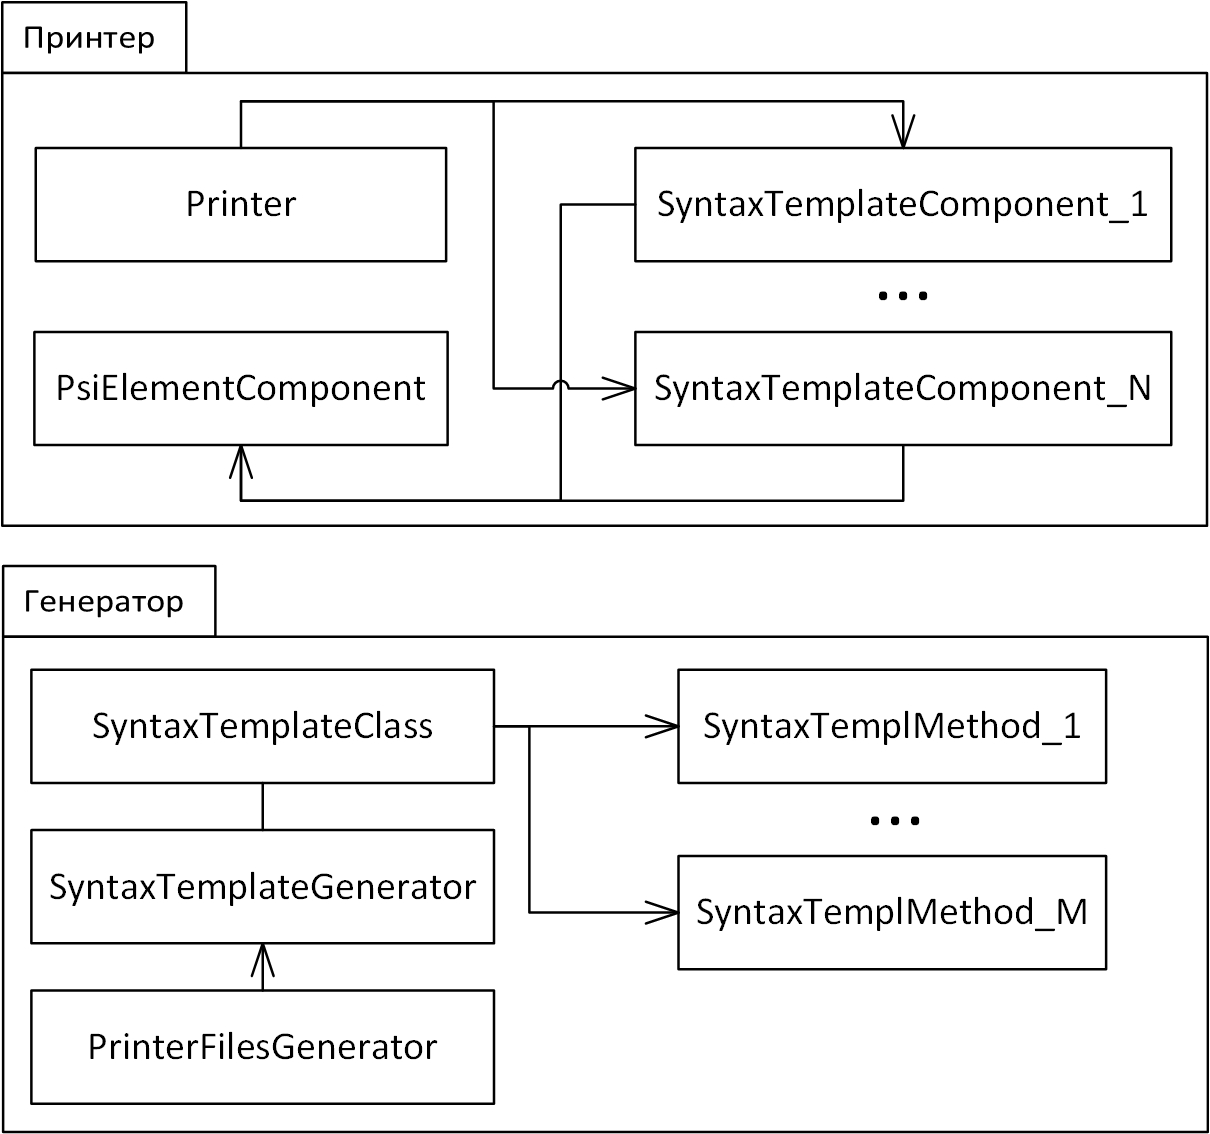
\includegraphics[width=0.75\linewidth]{Korovyansky/SystemArchitecture.jpg}}
\caption{Архитектура принтера и генератора}
\label{fig:Architecture}
\end{figure}

\subsection{Принтер для языка Java}
В первую очередь было решено сгенерировать принтер для языка Java. Поскольку изначально нам был доступен принтер для этого же языка, можно проверить корректность сгенерированного принтера используя те же тесты, что были созданы для исходного принтера. Новые же тесты также можно использовать для исходного и сгенерированного принтера. Более того, можно оценить насколько код, созданный генератором, отличается от кода исходного принтера.

Используя возможности созданного генератора были заданы XML-файлы для большинства компонент языка Java. Без написания дополнительного программного кода в XML-файлах возможна генерация большинства компонент без списочных поддеревьев. Исключениями являются структуры, в которых необходимо осуществлять дополнительную проверку корректности применения шаблона. В таких структурах недостаточно набора меток шаблона для его однозначной идентификации. Обычно эта дополнительная проверка требуется в структурах, которые определены в синтаксическом анализаторе слишком общно или неопределены вовсе\footnote{Множество таких примеров были обнаружены при создании принтера для языка Haskell, поскольку синтаксический анализатор, с которым велась работа, имел ряд ограничений.}.

Структуры, которые содержат списочные поддеревья должны обрабатываться особым образом, поэтому их методы обработки определены не так же, как в большинстве компонент. Из-за этого их генерация невозможна без написания дополнительного кода в XML-файлах. В худшем случае приходится полностью описывать новые методы обработки в XML-файлах. По аналогичным соображениям невозможна простая генерация структуры ``\lstinline{try-catch}'' и структуры, отвечающей за арифметические выражения.

Существует ряд структур, обработка которых была специально упрощена для ускорения работы принтера. Обычно в таких структурах невозможна обработка поддеревьев перед обработкой самой структуры. Например, у структуры ``\lstinline{switch}'' невозможно задать оптимальный вариант форматирования всех поддеревьев ``\lstinline{case}'' без анализа самой структуры ``\lstinline{switch}''. Одним из вариантов упрощения является явное задание форматирования. Это противоречит концепции принтеров, с которыми мы работаем, но при этом ускоряет их работу~\cite{podkopaev:diploma} и позволяет вести их генерацию без включения программного кода в XML-файлы.

В результате было создано множество XML-файлов, по которым возможна генерация принтера для языка Java. Сгенерированный принтер и исходный были проверены общим множеством тестов, признанным нами достаточным, посколько оно покрывает большинство структур языка. Результаты тестов были идентичны для исходного и сгенерированного принтеров, что предсказуемо, поскольку код сгенерированного принтера для языка Java должен быть эквивалентен исходному коду оригинального принтера, но с развернутой иерархией классов.

Также был проведен анализ производительности сгенерированного принтера. Основной целью анализа является сравнение времени работы сгенерированного принтера и оригинального, написанного вручную. Результаты анализа приведены в таблице~\ref{JavaPerformanceTbl}. Для каждого теста было выполнено 10 изменерений. Для тестирования рассматривались исходные файлы проекта IntelliJ IDEA Community Edition\footnote{\url{http://github.com/jetbrains/intellij-community}}.  В таблице указаны среднее время форматирования сгенерированным принтером (Время (A)), стандартное отклонение среднего результата сгенерированного принтера (Откл. (A)), среднее время форматирования оригинальным принтером (Время (B)), стандартное отклонение среднего результата оригинального принтера (Откл. (B)). Все тесты были проведены на одном и том же устройстве.

\begin{table}[H]
\begin{center}
{\scriptsize
\begin{tabular}{|c|c|c|c|c|c|}
\hline
Название файла & Кол-во строк & Время (A) & Откл. (A) & Время (B) & Откл. (B)\\
\hline
QuickEditHandler.java & 504 & 232.7 & 19.4 & 212.2 & 17.3\\
UIUtil.java & 2808 & 1131.2 & 21.9 & 1157.5 & 25.8\\
AbstractTreeUi.java & 5112 & 1703.7 & 25.1 & 1624.0 & 22.8\\
EditorImpl.java & 6789 & 2045.0 & 28.9 & 2079.6 & 26.2\\
ConcurrentHashMap.java & 7191 & 1286.2 & 20.5 & 1384.4 & 21.2\\
\hline
\end{tabular}}
\end{center}
\caption{\label{JavaPerformanceTbl}Время форматирования файлов (в миллисекундах)}
\end{table} 

Исходя из представленных результатов, можно сделать вывод, что время работы оригинального и сгенерированного принтеров практически совпадает. Это еще раз подтверждает, что код сгенерированного принтера эквивалентен исходному.

\subsection{Принтер для языка Haskell}

Для дальнейшего тестирования было решено разработать принтер для языка Haskell на основе описанного подхода. В языке Haskell имеется множество отличных от Java структур, что позволяет проверить выразительность нашей системы описания шаблонов. Более того, двумерный синтаксис языка является дополнительным испытанием для работы принтера. Основной же целью генерации принтера для языка Haskell была именно апробация метода генерации, то есть проверка при каких условиях генерация и сам алгоритм принтера будут работать корректно, а также какие существуют ограничения у разработанного метода и как их можно преодолеть. 

Для начала работы необходимо было выбрать реализованный синтаксический анализатор для языка Haskell. Поскольку мы используем генерируемые принтеры в качестве плагинов к среде IntelliJ IDEA, было решено использовать плагин для поддержки языка Haskell для этой среды разработки. Существуют два альтернативных плагина: разработанный компанией Jetbrains на языке Kotlin\footnote{\url{https://github.com/Atsky/haskell-idea-plugin}} и неофициальный, написанный на языке Scala\footnote{\url{https://github.com/rikvdkleij/intellij-haskell}}. Оба плагина содержат реализованный синтаксический анализатор и пригодны для работы в принтере. Для генерации был выбран официальный плагин, поскольку архитектура его анализатора схожа с синтаксическим анализатором, который был использован для генерации принтера языка Java. При этом критерий качества синтаксического анализатора не является значимым для выбора, так как, при наличии неточностей у анализатора, могут быть выявлены ограничения у разработанного метода, что является одной из основных целей апробации. 

Первой преградой для генерации стала фабрика элементов языка, то есть класс, отвечающий за создание новых экземпляров структур из их текстового представления. Для плагина языка Haskell было достаточно лишь возможности создавать экземпляр класса ``файл языка Haskell''. Для принтера необходима возможность создания из текста любой структуры языка. Было решено расширить функционал фабрики, добавив методы для создания основных структур языка. Некоторые структуры возможно создавать в качестве поддеревьев основных структур. Например, любое выражение из его текстового представления можно получить следующим образом:

\begin{itemize}
\item добавить в начало текстового представления выражения, например, ``\lstinline{temp = }'';
\item создать из получившегося текстового представления структуру присваивания\footnote{Предполагается, что метод создания из текстового представления структуры присваивания уже реализован};
\item выделить правое поддерево структуры присваивания, что и будет целевым выражением.
\end{itemize}

Во время этой обработки проявляется одно из основных отличий языка Haskell от языка Java~--- двумерный синтаксис. Если в Java синтаксическая корректность структуры не может быть нарушена подобными добавлениями в текстовое представление, то в Haskell это добавление сдвинет первую строчку выражения, что приведет к некорректности многострочного выражения (рис.~\ref{haskellFormatSamples}.a).

\fvset{frame=lines,framesep=5pt}
\begin{figure}[ht]
\noindent\begin{minipage}{.25\textwidth}
    \begin{lstlisting}[language=Haskell,basicstyle=\scriptsize]
temp = let y = 1+3
       z = 1+2
       in  z+y
    \end{lstlisting}
\caption*{a)}    
\end{minipage}\hfill
\begin{minipage}{.40\textwidth}
    \begin{lstlisting}[language=Haskell,basicstyle=\scriptsize]
temp = let y = 1+3
           z = 1+2
                  in  z+y 
    \end{lstlisting}
\caption*{b)}    
\end{minipage}\hfill
\begin{minipage}{.25\textwidth}
    \begin{lstlisting}[language=Haskell,basicstyle=\scriptsize]
temp = let y = 1+3
           z = 1+2
           in  z+y
    \end{lstlisting}
\caption*{c)}    
\end{minipage}
\caption{Применение различных вариантов сдвига к структуре ``\lstinline{let}'' языка Haskell}    
\label{haskellFormatSamples}
\end{figure}

Таким образом, прежде чем добавить что-либо к текстовому представлению необходимо его построчно сдвинуть. К сожалению, обычный построчный сдвиг может привести к некорректному результату форматирования. Например, в структуре ``\lstinline{let}'' языка Haskell присутствует ключевое слово \lstinline{in}, которое никак не выделяется синтаксическим анализатором. Сдвиг данной строчки не обязан совпадать с остальными выражениями структуры ``\lstinline{let}''. Дополнительный отступ этой строки будет интерпретироваться как часть форматирования структуры ``\lstinline{let}'', что приведет к некорректному отступу этой строки в отформатированном коде (рис.~\ref{haskellFormatSamples}.b). В результате был добавлен функционал ``умного'' сдвига, позволяющий избежать данной проблемы (рис.~\ref{haskellFormatSamples}.c). 

В ходе работы с плагином был обнаружен ряд особенностей реализованного синтаксического анализатора. Во-первых, некоторые структуры невозможно идентифицировать в контексте анализатора. Например, структура ``\lstinline{if}'' разпознается как три экземпляра структуры ``выражения''. Так же распознается и структура ``список'' содержащая три элемента--``выражения''. То есть в контекте синтаксического анализатора эти структуры неотличимы (рис.~\ref{haskellAnalyzerIncorrect}). Во-вторых, уже упомянутые ``списки'' не распознаются как отдельный элементы. Синтаксический анализатор возвращает лишь набор элементов, содержащихся в них, но не структуры ``список''. Это полностью исключает возможность переиспользования решения для списков, написанного для языка Java.

\fvset{frame=lines,framesep=5pt}
\begin{figure}[H]
    \begin{lstlisting}[language=Haskell]
    tmp1 a b = if (a && b) then (a && True) else (b && True)
    tmp2 a b = [(a && b), (a && True), (b && True)]
    \end{lstlisting}
\caption{Неотличимые структуры с точки зрения синтаксического анализатора, с которым велась работа}   
\label{haskellAnalyzerIncorrect}
\end{figure}

В исходном принтере были реализованы два варианта работы со списочными элементами. Первый алгоритм задает фиксированный разделитель элементов, который используется для их ``склейки''. Это противоречит концепции принтеров, с которыми мы работаем, но при этом сохраняет линейность работы общего алгоритма.
Второй метод работает следующим образом. 

\begin{itemize}
\item Создается метод, выделяющий списочную структуру из текста.
\item Анализируя структуру можно выделить все местоположения разделителей элементов.
\item Каждый разделитель выделяется и сохраняется в специальный шаблон для списочных элементов. Этот шаблон позволяет между любыми соседними элементами списка вставить один из разделителей из набора выделенных. 
\end{itemize}

Второй способ для каждого списка из эталонного кода создаст по одному списочному шаблону, который фактически представляет из себя набор разделителей списка. Каждый такой шаблон может продуцировать множество вариантов списка, к которому был применен, размер которого может расти экспоненциально от количества элементов списка. Таким образом, второй способ имеет высокий уровень выразительности, но при этом достаточно трудоемок.

Для особой работы со списочными элементами был создан отдельный класс обработки. Каждый такой класс соответствует конкретному списочному элементу в синтаксическом анализаторе. Если же в синтаксическом анализаторе нет элемента, который соответствует некоторой списочной структуре, то существующим решением невозможно корректно его обрабатывать. 

Используемый синтаксический анализатор распознает две структуры списочного типа: ``тип элемента~--- список'', ``тип элемента~--- кортеж'' (рис.~\ref{haskellTypes}). Для них было реализовано решение, подобное описанному для языка Java.

\fvset{frame=lines,framesep=5pt}
\begin{figure}[H]
    \begin{lstlisting}[language=Haskell]
    tmp1 :: [A,C]
    tmp2 :: (A,B,C)
    \end{lstlisting}
\caption{Структуры ``тип элемента~--- список'', ``тип элемента~--- кортеж''}   
\label{haskellTypes}
\end{figure}

Также проявилась проблема группировки поддеревьев. Методы выделения поддеревьев структуры возвращают наборы поддеревьев одного типа, после чего форматируют все полученные наборы отдельно и конкатенируют результат. Таким образом, во время форматирования поддеревья группируются, и в результате их порядок может отличаться от исходного (рис.~\ref{haskellModule}). Для решения было предложено все полученные наборы поддеревьев объединять в один, после чего отсортировать элементы по их местоположению в исходном тексте, тем самым восстанив их порядок. После этого объединенному набору присваивается одна метка, и задача сводится к обработке списочного элемента. 

В результате работы был сгенерирован принтер для языка Haskell, корректность которого была проверена рядом тестов, признанным нами достаточным. Также были выявлены ограничения генерации и ограничения принтера. Во-первых, для корректной работы генератора необходимо наличие в фабрике элементов языка методов для создания любого элемента из его текстового представления. Во-вторых, при использования второго метода работы со списочными поддеревьями, без дополнительной обработки невозможна генерация классов описания шаблонов для списочных структур. В-третьих, проблема обработки элементов с нефиксированным набором поддеревьев также остается нерешенной в общем случае, поэтому генерация подобных конструкций невозможна без дополнительной обработки.

В контексте поставленной задачи целесообразно сравнить производительность сгенерированного принтера для языка Haskell и существующих аналогов. Это позволит оценить насколько функционал, предоставляемый сгенерированным принтером, трудоемок по сравнению с существующими системами форматирования языка Haskell. Файлы для тестирования взяты из репозитория bitemyapp/hackage-packages\footnote{\url{https://github.com/bitemyapp/hackage-packages}}. 

Для сравнения в первую очередь рассматривались решения включенные в среду разработки IntelliJ IDEA, но готовых реализаций принтеров для языка Haskell в ней не предусмотрено. Поэтому в качестве аналога был использован принтер из пакета haskell-src-exts\footnote{\url{http://hackage.haskell.org/package/haskell-src-exts}}. Этот принтер был выбран нами, поскольку он является одним из базовых решений для языка Haskell и используется во многих существующих проектах\footnote{\url{http://goo.gl/zWSzPN}}. Он позволяет форматировать исходный код лишь в изначально прописанном стиле. Изменить заданный стиль нельзя, необходимо полностью переписывать принтер. 

В тестах измерено время этапа форматирования кода. Время выделения шаблонов из идеального образца не представляет интереса, поскольку в практике должно быть выполнено один раз и после этого будет осуществлятся лишь форматирование по выделеному стилю. Результаты производительности приведены в
таблице~\ref{HaskellPerformanceTbl}. Для каждого теста было выполнено 10 изменерений. В таблице указаны среднее время форматирования сгенерированным принтером (Время (A)), стандартное отклонение среднего результата сгенерированного принтера (Откл. (A)), среднее время форматирования принтером пакета haskell-src-exts (Время (B)), стандартное отклонение среднего результата сгенерированного принтера пакета haskell-src-exts (Откл. (B)). Все тесты были проведены на одном и том же устройстве.

\begin{table}[H]
\begin{center}
{\scriptsize
\begin{tabular}{|c|c|c|c|c|c|}
\hline
Название файла & Кол-во строк & Время (A) & Откл. (A) & Время (B) & Откл. (B)\\
\hline
HughesPJ.hs & 997 & 465.5 & 15.5 & 186.2 & 19.6\\
TraceTrans.hs & 2723 & 914.5 & 17.5 & 331.0 & 19.0\\
TimeBuiltinTypes.hs & 4406 & 1970.5 & 13.5 & 596.7 & 28.6\\
ResolveOperators.hs & 7109 & 1462 & 18.6 & 546.2 & 17.7\\
Lojban.hs & 11735 & 2982.8 & 98.3 & 979.9 & 25.7\\
\hline
\end{tabular}}
\end{center}
\caption{\label{HaskellPerformanceTbl}Время форматирования файлов (в миллисекундах)}
\end{table} 

Исходя из представленных данных можно сделать вывод, что сгенерированный принтер работает медленнее своего аналога. Этот результат достаточно ожидаем, так как сгенерированный принтер при форматировании конструкций должен просматривать множество синтаксических шаблонов. Время работы сгенерированного принтера обладает сильной зависимостью от содержимого обрабатываемых файлов, а точнее от форматируемых конструкций в файле. Например, если в нем содержится множество элементов списочного типа, то его обработка будет проходить медленее чем обработка файлов, не содержащих таких структур, но с таким же количество строк~\cite{podkopaev:diploma}. Файл ``TimeBuiltinTypes.hs'' состоит из 26 объявлений новых структур. В контексте синтаксического анализатора эти элементы являются списками, и именно этим обуславливается временной скачок при работе с файлом ``TimeBuiltinTypes.hs''.

% У заключения нет номера главы
\section*{Заключение}
В ходе выполнения работы были получены следующие результаты.
\begin{itemize}
\item Предложена структура для генерации описаний синтаксических шаблонов.
\item Разработан генератор языкозависимой части принтеров. Генератор реализован на языке Kotlin в среде IntelliJ IDEA.
\item Выполнена реализация принтеров для языков Java, Haskell на основе сгенерированных описаний синтаксических шаблонов.
\end{itemize}

Код проекта находится на сайте \url{https://bitbucket.org/alexeykor/printerplugin}.


Ниже представлены направления для дальнейшей работы:

\begin{itemize}
\item Для увеличения множества генерируемых структур необходимо дальнейшее совершенствование описания шаблонов.
\item Необходима генерация принтеров для новых языков в качестве дополнительной апробации метода.
\item Иным направлением для развития является улучшение алгоритма работы принтеров. Предложенная реализация имеет ряд проблем при обработке структур определенного типа, например, списков и комментариев.
\end{itemize}

\begin{thebibliography}{99}
  \bibitem{podkopaev:course}
  A.В.Подкопаев. Форматирование текста программ на основе комбинаторов, сопоставления с 
  образцом и синтаксических шаблонов. Курсовая работа, кафедра системного программирования, 
  математико-механический факультет СПбГУ, 2013.

  \bibitem{podkopaev:diploma}
  A.В.Подкопаев. Полиномиальной сложности оптимальные принтер-комбинаторы с выбором.
  Дипломная работа, кафедра системного программирования, математико-механический факультет СПбГУ, 2014.

  \bibitem{podkopaev:english}
  A.Рodkopaev, D.Boulytchev. Polynomial-Time Optimal Pretty-Printing Combinators with Choice //
  Perspectives of System Informatics, 2015, P.~257--265.

  \bibitem{indentation}
    R.J.Miara, J.A.Musselman, J.A.Navarro, B.Shneiderman. Program Indentation and Comprehensibility //
    CACM, 1983, P.~861--867.

  \bibitem{artOfAgile}
    J.Shore. The Art of Agile Development. O’Relly Media, 2010.

  \bibitem{oppen}
    D.Oppen. "Prettyprinting // ACM Transactions on Programming Languages and Systems,
    Vol.~2, \textnumero~4, P.~465--483.

  \bibitem{oppenlike:rose}
    G.A.Rose, J.Welsh. Formatted Programming Languages // Software~--- Practice and Xxperience,
    Vol.~11, 1981, P.~651--669.

  \bibitem{oppenlike:mikelsons}
    M.Mikelsons. Prettyprinting in an Interactive Programming Environment //
    SIGPLAN Notices, Vol.~16, \textnumero~6, 1981, P.~108--116.

  \bibitem{oppenlike:rubin}
    L.F.Rubin. Syntax-Directed Pretty Printing~--- A First Step Towards a Syntax-Directed Editor //
    IEEE Transactions on Software Engineering, Vol.~SE-9, 1983, P.~119--127.

  \bibitem{oppenlike:morcos}
    E.Morcos-Chounet, A.Conchon. PPML: a General Formalism to Specify Prettyprinting //
    Information Processing, \textnumero~86, 1986, P.~583--590.

  \bibitem{oppenlike:brand}
    M.G.J.Brand, E.Visser. Generation of Formatters for Context-free Languages //
    ACM Transactions on Software Engineering and Methodology, Vol.~5, \textnumero~1, 1996,
    P.~1--41.

  \bibitem{oppenfunc:hughes}
    J.Hughes. The Design of a Pretty-Printing Library // Advanced Functional Programming,
    Vol.~925, 1995, P.~53--96.

  \bibitem{oppenfunc:swierstra}
    P.Azero, S.D.Swierstra. Optimal Pretty-Printing Combinators.
    \url{http://www.cs.ruu.nl/groups/ST/Software/PP}, 1998.

  \bibitem{oppenfunc:wadler}
    P.Wadler. A Prettier Printer // The Fun of Programming. Palgrave MacMillan, 2003.

  \bibitem{box:knuth}
    D.E.Knuth. TEX and METAFONT: New Directions in Typesetting //
    Digital Press and the American Mathematical Society, 1979.

  \bibitem{jokinen}
    M.O.Jokinen. A Language-Independent Prettyprinter // Software~--- Practice and Experience,
    Vol.~19, \textnumero~9, 1989, P.~839--856.

  \bibitem{boulton}
    R.J.Boulton.SYN: A Single Language for Specifying Abstract Syntax Trees, Lexical Analysis, 
    Parsing and Pretty-Printing. Technical Report, Computer Laboratory, University of Cambridge,
    1996.

  \bibitem{jonge}
    M.Jonge. A Pretty-Printer for Every Occasion. Centre for Mathematics and Computer Science,
    2001.

  \bibitem{jackson}
    S.Jackson. Stable, Flexible, Peephole Pretty-Printing // Science of Computer Programming,
    Vol.~72, \textnumero~1--2, 2008, P.~40--51.

  \bibitem{blaschek}
    G.Blaschek, J.Sametinger. User-adaptable Prettyprinting // Software~--- Practice and Experience,
    Vol.~19, 1989.
\end{thebibliography}
